\documentclass[aspectratio=169]{beamer}

% PACKAGES
\usepackage[french]{babel}
\usepackage[utf8]{inputenc}
\usepackage[T1]{fontenc}
\usepackage{graphicx}
\usepackage{tikz}
\usetikzlibrary{shapes,arrows,positioning,backgrounds,calc}

% COULEURS 
\definecolor{mainblue}{RGB}{0,66,130}      % Bleu Évry
\definecolor{lightblue}{RGB}{100,150,200}  % Bleu clair
\definecolor{darkgray}{RGB}{50,50,50}
\definecolor{lightgray}{RGB}{240,240,245}

% CONFIGURATION THÈME
\usetheme{default}
\useinnertheme{rectangles}
\setbeamertemplate{navigation symbols}{}

% Couleurs des éléments du thème
\setbeamercolor{structure}{fg=mainblue}
\setbeamercolor{frametitle}{bg=mainblue,fg=white}
\setbeamercolor{title}{fg=mainblue}
\setbeamercolor{block title}{bg=mainblue,fg=white}
\setbeamercolor{block body}{bg=lightgray,fg=darkgray}
\setbeamercolor{block title alerted}{bg=red!80!black,fg=white}
\setbeamercolor{block body alerted}{bg=red!10,fg=darkgray}
\setbeamercolor{block title example}{bg=lightblue,fg=white}
\setbeamercolor{block body example}{bg=lightblue!20,fg=darkgray}

% Items
\setbeamertemplate{itemize item}{\color{mainblue}$\blacktriangleright$}
\setbeamertemplate{itemize subitem}{\color{lightblue}$\bullet$}

% Pied de page : numérotation des diapositives
\setbeamertemplate{footline}{
  \hbox{%
    \begin{beamercolorbox}[wd=\paperwidth,ht=2.5ex,dp=1ex,right]{page number in head/foot}%
      \usebeamerfont{page number in head/foot}\insertframenumber{} / \inserttotalframenumber\hspace*{2ex}
    \end{beamercolorbox}%
  }%
  \vskip0pt%
}
% Informations principales : titre, auteur, date
\title{Les rêves à la lumière de l'informatique}
\subtitle{Entre neurosciences et intelligence artificielle}
\author{AZZOUZ Ilhem \and BELKACEMI Cirine \and BOURAKKADI IDRISSI Marwa}
\institute{Université d'Évry Paris-Saclay}
\date{24 Novembre 2024}

\begin{document}

% SLIDE 1 : PAGE DE GARDE
{ 
\setbeamercolor{page number in head/foot}{fg=white}
\setbeamertemplate{background}{
\begin{tikzpicture}[remember picture,overlay]
% Fond bleu foncé
\fill[mainblue!95!black] (current page.south west) rectangle (current page.north east);

\fill[white] (current page.north east) -- 
  ([xshift=-6cm]current page.north east) -- 
  ([yshift=-4cm]current page.north east) -- cycle;

% Logo en haut à DROITE 
\node[anchor=north east, xshift=-1cm, yshift=-0.3cm] at (current page.north east) {
  
\includegraphics[height=1.4cm]{LOGO_UNIV}
};
\end{tikzpicture}
}
\begin{frame}

\vfill

\begin{center}
\vspace{1.5cm} 

{\Huge\bfseries\color{white}Les rêves à la lumière de l'informatique}

\vspace{1cm} 

{\Large\itshape\color{white!90}Entre neurosciences et intelligence artificielle}

\vspace{1.2cm} 

\begin{columns}[T]
\column{0.33\textwidth}
\centering
{\large\color{white}AZZOUZ Ilhem}

\column{0.33\textwidth}
\centering
{\large\color{white}BELKACEMI Cirine}

\column{0.33\textwidth}
\centering
{\large\color{white}BOURAKKADI IDRISSI \\[-0.5ex] Marwa}
\end{columns}

\vspace{0.7cm}

{\large\color{white}24 Novembre 2025}
\end{center}


\vfill

\end{frame}
}


% SLIDE 2 : SOMMAIRE 
{
\setbeamertemplate{background}{
\begin{tikzpicture}[remember picture,overlay]
  \fill[mainblue] (current page.south west) rectangle (current page.north east);
\end{tikzpicture}
}

% Forcer la couleur blanche sur la zone du numéro de page
\setbeamercolor{page number in head/foot}{fg=white}

% Pied de page avec numéro dynamique blanc sur fond bleu
\setbeamertemplate{footline}{
  \hbox{%
    \begin{beamercolorbox}[wd=\paperwidth,ht=2.5ex,dp=1ex,right]{page number in head/foot}%
      \usebeamerfont{page number in head/foot}\insertframenumber{} / \inserttotalframenumber\hspace*{2ex}
    \end{beamercolorbox}%
  }%
}

\begin{frame}

\vspace{0.2cm}
\begin{minipage}{0.87\textwidth}
  {\LARGE\bfseries\color{white}Plan de la présentation}

  \vspace{0.8cm}

  {\large
  \begin{itemize}
    \item[] \hyperlink{introduction}{\color{white}$\blacktriangleright$ Introduction}
    \vspace{0.28cm}
    \item[] \hyperlink{perspectives}{\color{white}$\blacktriangleright$ Les rêves : une perspective scientifique}
    \vspace{0.28cm}
    \item[] \hyperlink{informatique}{\color{white}$\blacktriangleright$ Informatique et étude des rêves}
    \vspace{0.28cm}
    \item[] \hyperlink{simulation}{\color{white}$\blacktriangleright$ Simulation des rêves par l’intelligence artificielle}
    \vspace{0.28cm}
    \item[] \hyperlink{applications}{\color{white}$\blacktriangleright$ Applications concrètes}
    \vspace{0.28cm}
    \item[] \hyperlink{limites}{\color{white}$\blacktriangleright$ Limites et enjeux éthiques}
    \vspace{0.28cm}
    \item[] \hyperlink{conclusion}{\color{white}$\blacktriangleright$ Conclusion}
  \end{itemize}
  }
\end{minipage}

\end{frame}
}


% SLIDE 3 : INTRODUCTION 

\section{Introduction}

\begin{frame}{Introduction}\label{introduction}

\vspace{0.12cm}
\begin{itemize}
  \item Le rêve = activité mentale du sommeil    
  \item Présent à tous les stades du sommeil
  \item Étude par les neurosciences et l'informatique
  \item \textbf{Objectif :} comprendre, simuler, interpréter
\end{itemize}

\vspace{0.32cm}

\begin{exampleblock}{D. Oudiette (ICM)}
\small « Tout contenu mental qui se produit pendant le sommeil »
\end{exampleblock}

\vspace{0.38cm}

\begin{block}{Transition}
Comment la science explique-t-elle le rêve ?
\end{block}

\end{frame}

% SLIDE 4 : PERSPECTIVE SCIENTIFIQUE
\section{Perspectives scientifiques}\label{perspectives}

\begin{frame}{Les rêves : une perspective scientifique}

\begin{columns}[T]
\column{0.52\textwidth}

\begin{itemize}
  \item Se produisent surtout pendant le \textbf{sommeil paradoxal (REM)}
  \vspace{0.3cm}
  \item Activité cérébrale proche de l'éveil
  \vspace{0.3cm}
  \item \textbf{Outils :} EEG, IRMf → zones actives
  \vspace{0.3cm}
  \item Données pour la modélisation
\end{itemize}

\vspace{0.7cm}
\begin{exampleblock}{Matthew Walker (2017)}
\small « Le rêve est un laboratoire de simulation émotionnelle. »
\end{exampleblock}

\column{0.43\textwidth}
\centering

\vspace{0.22cm} 
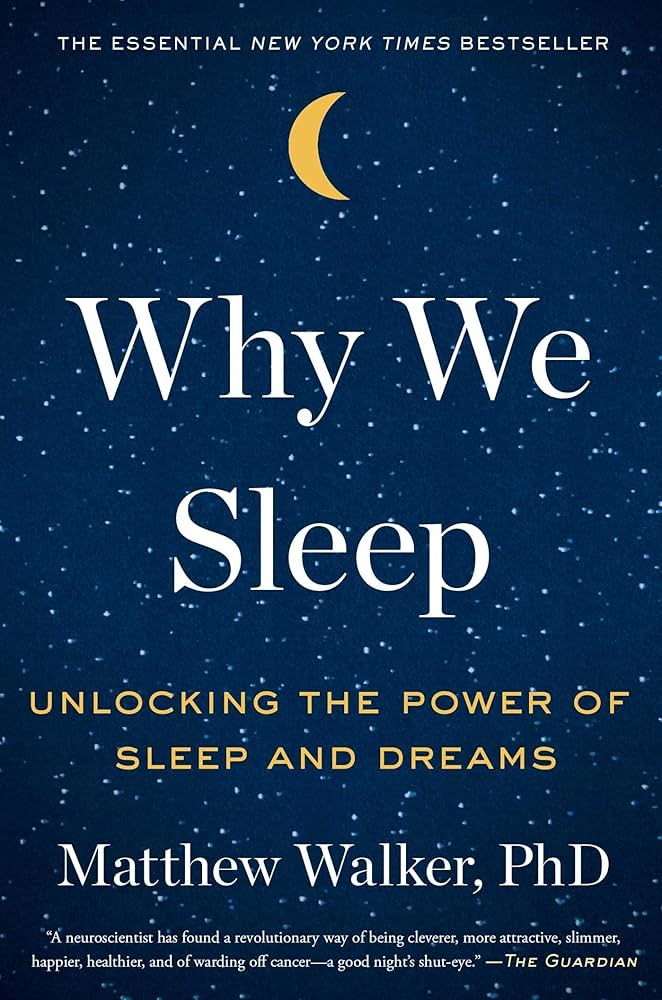
\includegraphics[width=0.65\textwidth]{why_we_sleep_cover.jpg}

\vspace{0.15cm} 
{\small\itshape Why We Sleep}

{\footnotesize Matthew Walker, 2017}

\end{columns}

\end{frame}

% SLIDE 5 :INFORMATIQUE ET RÊVES
\section{Informatique et rêves}

\begin{frame}{Informatique et étude des rêves}\label{informatique}

\begin{itemize}
  \item \textbf{Acquisition :} EEG, signaux cérébraux enregistrés
  
  \vspace{0.4cm}
  
  \item \textbf{Traitement :} détection automatique des phases de sommeil
  
  \vspace{0.4cm}
  \item \textbf{IA / Machine Learning :} prédiction émotions ou contenus
  
  \vspace{0.4cm}
  
  \item Étude Arte (2020) : IA traduisant signaux neuronaux en images
  
  \vspace{0.4cm}
  
  \item Collaboration entre neurosciences et intelligence artificielle
\end{itemize}

\vspace{0.8cm}

\begin{block}{Transition}
Et si l'IA pouvait « rêver » à son tour ?
\end{block}

\end{frame}
% SLIDE 6 : SIMULATION PAR IA
\section{Simulation par l'IA}

\begin{frame}{Simulation des rêves par l'IA} \label{applications}\label{simulation}

\textbf{Simulation :}

\begin{itemize}
  \item GANs / DeepDream → images oniriques créées par IA
  \item BBC (2021) : reconstruction visuelle des rêves réels
  \item L'IA explore des combinaisons nouvelles d'informations
  \item Une forme de « créativité artificielle »
\end{itemize}

\vspace{0.5cm}

\textbf{Applications :}

\begin{itemize}
  \item    Détection automatique des troubles du sommeil
  \item    Interprétation psychologique assistée par IA
  \item    Art numérique : visuels inspirés des rêves
  \item    Interfaces cerveau-machine : reconstruction d'images mentales
\end{itemize}

\end{frame}

% SLIDE 7 : LIMITES ÉTHIQUES 

\section{Limites éthiques}

\begin{frame}{Limites et enjeux éthiques} \label{limites}

\begin{itemize}
  \item    \textbf{Vie privée :} les signaux cérébraux = données personnelles
  \vspace{0.4cm}
  \item ⚖ \textbf{Éthique :} peut-on « lire » les pensées sans accord ?
  \vspace{0.4cm}
  \item    \textbf{Fiabilité :} les IA ne reproduisent pas la complexité émotionnelle
\end{itemize}

\vspace{0.8cm}

% Citation Jean-Michel Besnier style bleu clair
\begin{exampleblock}{Jean-Michel Besnier (2010)}
\small « À force de vouloir pénétrer l'intime du rêve, l'homme risque d'oublier le mystère de sa conscience. »
\end{exampleblock}

\vspace{0.5cm}

\begin{block}{Question ouverte}
Jusqu'où peut-on aller ?
\end{block}

\end{frame}

% SLIDE 8 : CONCLUSION

\section{Conclusion}

\begin{frame}{Conclusion}\label{conclusion}

\begin{itemize}
  \item Le rêve : un champ \textbf{interdisciplinaire}
  
  \vspace{0.3cm}
  
  \item L'IA + neurosciences = nouvelles perspectives
  
  \vspace{0.3cm}
  
  \item Vers une meilleure compréhension du cerveau et de la conscience
  
  \vspace{0.3cm}
  
  \item L'informatique transforme le mystère en objet d'étude
\end{itemize}

\vspace{0.8cm}

\begin{block}{Ouverture}
\begin{itemize}
  \item Lecture des pensées ?
  \item Rêves artificiels personnalisés ?
\end{itemize}
\end{block}

\end{frame}

% SLIDE 9 : REMERCIEMENTS
{
\setbeamercolor{page number in head/foot}{fg=white}

\setbeamertemplate{background}{
\begin{tikzpicture}[remember picture,overlay]
% Fond bleu foncé
\fill[mainblue!95!black] (current page.south west) rectangle (current page.north east);

% Triangle blanc dans le coin supérieur droit
\fill[white] (current page.north east) -- 
  ([xshift=-6cm]current page.north east) -- 
  ([yshift=-4cm]current page.north east) -- cycle;

% Logo 
\node[anchor=north east, xshift=-1cm, yshift=-0.3cm] at (current page.north east) {
  
\includegraphics[height=1.4cm]{LOGO_UNIV}
};
\end{tikzpicture}
}
\begin{frame}\label{remerciements}

\vfill

\begin{center}
\vspace{2.5cm}

{\Huge\bfseries\color{white}Merci de votre attention~!}

\vspace{1.8cm}

{\LARGE\color{white}Des questions ?}

\vspace{3cm}

\end{center}

\vfill

\end{frame}
}

\end{document}